\documentclass[12pt]{extarticle}
\usepackage[english,ukrainian]{babel}
\usepackage[utf8]{inputenc}
\usepackage{amsmath,amssymb}
\usepackage{parskip}
\usepackage{graphicx}
\usepackage{xcolor}
\usepackage{tcolorbox}
\tcbuselibrary{skins}
\usepackage[framemethod=tikz]{mdframed}
\usepackage{chngcntr}
\usepackage{enumitem}
\usepackage{hyperref}
\usepackage{float}
\usepackage{subfig}
\usepackage{chngcntr}
\usepackage{esint}

\usepackage[top=2.5cm, left=3cm, right=3cm, bottom=4.0cm]{geometry}
\usepackage[table]{xcolor}

\usepackage{algorithm}
\usepackage{algpseudocode}
\usepackage{listings}
\usepackage{xcolor}
\usepackage{dsfont}

\definecolor{codegreen}{rgb}{0,0.6,0}
\definecolor{codegray}{rgb}{0.5,0.5,0.5}
\definecolor{codepurple}{rgb}{0.58,0,0.82}
\definecolor{backcolour}{rgb}{0.95,0.95,0.92}

\lstdefinestyle{mystyle}{
    backgroundcolor=\color{backcolour},   
    commentstyle=\color{codegreen},
    keywordstyle=\color{magenta},
    numberstyle=\tiny\color{codegray},
    stringstyle=\color{codepurple},
    basicstyle=\ttfamily\footnotesize,
    breakatwhitespace=false,         
    breaklines=true,                 
    captionpos=b,                    
    keepspaces=true,                 
    numbers=left,                    
    numbersep=5pt,                  
    showspaces=false,                
    showstringspaces=false,
    showtabs=false,                  
    tabsize=2
}
\lstset{style=mystyle}

\usepackage{ragged2e}
\begin{document}

\begin{titlepage}
	\centering
	
\includegraphics[width=0.15\textwidth]{images/lab_1/logo.png}\par\vspace{0.3cm}
	{\textbf{Міністерство освіти і науки України}\par
 Харківський національний університет імені В.Н. Каразіна\par}
    \vspace{1cm}
	{\Large \textsc{Лабораторна робота \#3}\par
    \textbf{Середньоквадратичне наближення функцій алгебраїчними многочленами}\par}
	\vfill
 \begin{FlushRight}
	\textbf{Виконав:}\par Захаров Дмитро Олегович \par Група МП-31
\end{FlushRight}
	\vfill

% Bottom of the page
	{\large Харків -- 2023\par}
\end{titlepage}

\tableofcontents
\pagebreak

\section{Постановка задачі}

За даними з таблиці побудувати середньоквадратичне наближення функції, заданої таблично, алгебраїчним багаточленом третього ступеня.

Обчислити значення побудованого кубічного багаточлена у вузлах таблиці та оцінити похибку середньоквадратичного наближення.

На друк вивести результати у вигляді таблиць:
\[
x_i \; \; \; \; \; y_i \; \; \; \; \; f(x_i) \; \; \; \; \; |y_i-f(x_i)|,
\]
а також $\Delta$ -- відносну похибку середньоквадратичного наближення.

\textbf{Варіант 5.} 
\begin{center}
\begin{tabular}{ |c|c|c|c|c|c|c|c|c|c|c| } 
 \hline
 $y$ & 0.8 & 1.2 & 1.6 & 2.0 & 2.4 & 2.8 & 3.2 & 3.6 & 4.0 & 4.4 \\ \hline 
 $x$ & 1.97 & 3.53 & 3.57 & 2.42 & 2.44 & 1.30 & 0.71 & 2.12 & 3.08 & 5.99 \\ 
 \hline
\end{tabular}
\end{center}

\pagebreak
\section{Опис методу}

\subsection{Класична перспектива}\label{section:classical_method}
Нехай ми шукаємо апроксимацію у вигляді:
\[
f(x;\mathbf{w}) = \mathbf{w}^{\top}\boldsymbol{\phi}(x)
\]
де $\mathbf{w} \in \mathbb{R}^{m+1}$ -- вектор ваг, $\boldsymbol{\phi}(x) = \begin{bmatrix}
    1 & x & x^2 & \dots & x^m
\end{bmatrix}^{\top}$. 

Нехай ми маємо таблицю $\mathcal{D} = \{(x_i,y_i)\}_{i=1}^{n_{\mathcal{D}}} \subset \mathbb{R} \times \mathbb{R}$, яку ми хочемо апроксимувати.
Суть середньоквадратичної помилки -- оптимізувати функцію втрати:
\[
\hat{\mathbf{w}} = \arg\min_{\mathbf{w}}\mathcal{L}(\mathbf{w} \mid \mathcal{D}), \; \text{де} \; \mathcal{L}(\mathbf{w} \mid \mathcal{D}) \triangleq \sum_{i=1}^{n_{\mathcal{D}}} (f(x_i;\mathbf{w}) - y_i)^2
\]
Набір данних легше зобразити у вигляді матриці:
\[
\mathbf{X} = \begin{bmatrix}
    \boldsymbol{\phi}(x_1)^{\top} \\
    \boldsymbol{\phi}(x_2)^{\top} \\
    \vdots \\
    \boldsymbol{\phi}(x_{n_{\mathcal{D}}})^{\top}
\end{bmatrix} \in \mathbb{R}^{n_{\mathcal{D}} \times (m+1)}, \; \mathbf{y} = \begin{bmatrix}
    y_1 \\ y_2 \\ \vdots \\ y_{n_{\mathcal{D}}}
\end{bmatrix} \in \mathbb{R}^{n_{\mathcal{D}}}
\]
Тоді, наша задача еквівалентна
\[
\hat{\mathbf{w}} = \arg\min_{\mathbf{w}}\|\mathbf{y} - \mathbf{X}\mathbf{w}\|_2^2 = \arg\min_{\mathbf{w}}(\mathbf{y}-\mathbf{Xw})^{\top}(\mathbf{y}-\mathbf{Xw})
\]
Помітимо, що екстремум можна знайти за допомогою:
\[
\frac{\partial\mathcal{L}(\mathbf{w} \mid \mathcal{D})}{\partial \mathbf{w}} = 0 \iff \frac{\partial(\mathbf{y}^{\top}\mathbf{y} - \mathbf{y}^{\top}\mathbf{X}\mathbf{w}-\mathbf{w}^{\top}\mathbf{X}^{\top}\mathbf{y} + \mathbf{w}^{\top}\mathbf{X}^{\top}\mathbf{X}\mathbf{w})}{\partial\mathbf{w}}=0
\]
Після диференціювання, отримуємо:
\[
-2\mathbf{X}^{\top}\mathbf{y} + 2\mathbf{X}^{\top}\mathbf{Xw} = 0 \implies \boxed{\hat{\mathbf{w}} = (\mathbf{X}^{\top}\mathbf{X})^{-1}\mathbf{X}^{\top}\mathbf{y}} 
\]

\subsection{Ймовірнісна перспектива}
Нехай ми вважаємо, що функція $f(x;\mathbf{w})$, наведена у попередньому розділі \ref{section:classical_method}, найкраще апроксимує набір данних $\mathcal{D}$. В такому разі будемо вважати, що джерело різниці між реальними значеннями і ``теоретично'' правильними -- це гаусовий гум $\epsilon$, тобто:
\[
y = f(x;\mathbf{w}) + \epsilon, \; \text{де} \; \epsilon \sim \mathcal{N}(0,\sigma^2)
\]
В такому разі, умовна умовірність зустріти значення $y$ при заданому $x$:
\[
p(y \mid x) = \frac{1}{\sqrt{2\pi}\sigma}\exp\left\{-\frac{(y-f(x;\mathbf{w}))}{2\sigma^2}\right\}
\]
Нам потрібно знайти $\arg\max_{\mathbf{w}} p(\mathbf{y} \mid \mathbf{X})$, тобто максимізувати ймовірність мати увесь набір данних. Тобто:
\[
\hat{\mathbf{w}} = \arg\max_{\mathbf{w}} \prod_{i=1}^{n_{\mathcal{D}}}p(y_i \mid x_i)
\]
Проте, знаходити максимум від добутку не дуже зручно, тому помітимо, що ми можемо оптимізовувати замість цього так званий \textit{negative log-likelihood}:
\[
\hat{\mathbf{w}} = \arg\min_{\mathbf{w}}\left(-\log \prod_{i=1}^{n_{\mathcal{D}}}p(y_i\mid x_i)\right) = \arg\min_{\mathbf{w}}\left(\frac{n_{\mathcal{D}}}{2}\log 2\pi\sigma^2 + \frac{1}{2\sigma^2}\sum_{i=1}^{n_{\mathcal{D}}}(y_i-f(x_i;\mathbf{w}))^2\right)
\]
Оскільки $\frac{n_{\mathcal{D}}}{2}\log 2\pi \sigma^2$ ніяк не залежить від $\mathbf{w}$, то задача на оптимізацію еквівалентна:
\[
\hat{\mathbf{w}} = \arg\min_{\mathbf{w}} \sum_{i=1}^{n_{\mathcal{D}}} (y_i-f(x_i;\mathbf{w}))^2,
\]
що еквівалентно оптимізації у минулому пункті. 

\subsection{Оцінка точності}
Після того, як ми отримали коефіцієнти $\hat{\mathbf{w}}$, ми можемо оцінити відносну похибку за формулою:
\[
\Delta^2 = 
\frac{\sum_{i=1}^{n_{\mathcal{D}}}
(y_i-f(x_i;\hat{\mathbf{w}}))^2}{\sum_{i=1}^{n_{\mathcal{D}}}
y_i^2}
\]
Або, на мові попередніх розділів,
\[
\Delta = \frac{\|\mathbf{y}-\mathbf{X}\hat{\mathbf{w}}\|_2}{\|\mathbf{y}\|_2}
\]

\pagebreak
\section{Текст програми}

Повний текст програми можна знайти за \href{https://github.com/ZamDimon/University-Homeworks/tree/main/Term%205/Numerical%20Analysis/code/lab_3}{цим посиланням} ($\leftarrow$ напис клікабельний) на \textit{GitHub} сторінку.


\subsection{Пошук коефіцієнтів}

Створимо файл \texttt{solver.py} та реалізуємо алгоритм з розділу \ref{section:classical_method} у класі \texttt{LeastSquaresSolver}. При ініціалізації ми будемо вказувати ступінь полінома за яким ми хочемо апроксимувати, а також додамо 2 методи:
\begin{enumerate}
    \item \texttt{fit}: приймає набір данних $\mathcal{D}$ і повертає набір коефіцієнтів $\hat{\mathbf{w}}$ (а також зберігає їх в самому класі);
    \item \texttt{predict}: приймає $x\in \mathbb{R}$ і повертає $\hat{\mathbf{w}}^{\top}\boldsymbol{\phi}(x)$, тобто значення полінома зі знайденими коефіцієнтами у вказаній точці.
\end{enumerate}

\begin{lstlisting}[language=Python, caption=Реалізація пошуку коефіцієнтів методом найменших квадратів]
from typing import TypeAlias, Tuple, List
import numpy as np

Point: TypeAlias = Tuple[float, float]
Dataset: TypeAlias = List[Point]

class LeastSquaresSolver:
    """
    A class to solve the least squares problem
    """
    
    def __init__(self, degree: int) -> None:
        """
        Args:
            dataset (Dataset): A list of points
            degree (int): The degree of the polynomial to fit
        """
        
        self._degree = degree

    def _generate_power_vector(self, x: float) -> List[float]:
        """ Generates a row consisting of powers of x
        
        Args:
            x (float): The x value of the point
        
        Returns:
            List[float]: A row for the dataset matrix
        """
        
        return [x**i for i in range(self._degree + 1)]

    def fit(self, dataset: Dataset) -> np.ndarray:
        """ Returns a list of coefficients for the polynomial of the given degree
        
        Returns:
            np.ndarray: A list of coefficients for the polynomial of the given degree (degree + 1)
        """
        
        X = np.empty((len(dataset), self._degree + 1))
        Y = np.empty((len(dataset), 1))
        
        for i in range(len(dataset)):
            x, y = dataset[i]
            X[i] = self._generate_power_vector(x)
            Y[i] = y
                
        self._coefficients = np.linalg.inv(X.T @ X) @ X.T @ Y
        self._coefficients = np.squeeze(self._coefficients, axis=-1)
        return self._coefficients
    
    def predict(self, x: float) -> np.floating:
        """ Predicts the y value for the given x value
        
        Args:
            x (float): The x value to predict the y value for
        
        Returns:
            float: The predicted y value
        """
        
        return self._coefficients @ self._generate_power_vector(x)
\end{lstlisting}

\subsection{Програма запуску}

При запуску, ми робимо наступні дії:
\begin{enumerate}
    \item Ініціалізуємо \texttt{LeastSquaresSolver} та запускаємо \texttt{fit} метод на обраному наборі данних.
    \item Будуємо графік, де зображуємо поліном та точки з набору данних.
    \item Будуємо графік для різних ступенів поліному для перевірки.
    \item Будуємо таблицю, котру потребує завдання.
    \item Оцінюємо відносну похибку $\Delta$.
\end{enumerate}

Отже, наводимо код знизу (файл \texttt{main.py}), котрий робить вищезгадані кроки.

\begin{lstlisting}[language=Python, caption=Запуск методу найближчих квадратів]
import matplotlib.pyplot as plt
import matplotlib.patches as mpatches
import numpy as np
from typing import List

# Rich logging
from rich import print
from rich.console import Console
from rich.table import Table

from solver import LeastSquaresSolver, Dataset

def _show_predictions(dataset: Dataset, solver: LeastSquaresSolver) -> None:
    """ Shows the predictions of the fitted polynomial

    Args:
        dataset (Dataset): A list of points
        solver (LeastSquaresSolver): A LeastSquaresSolver instance
    """
    
    # Initializing an instance of rich.Table to make an attractive table in the console
    console = Console()
    table = Table(title='Degree vs real values for a linear regression')
    table.add_column('x', justify='center', style='white')
    table.add_column('y', justify='center', style='green')
    table.add_column('f(x)', justify='center', style='blue')
    table.add_column('|y - f(x)|', justify='center', style='red')
    
    # Adding rows to the table
    for (x, y) in dataset:
        x_label = '{:.8f}'.format(x)
        y_label = '{:.8f}'.format(y)
        prediction_label = '{:.8f}'.format(float(solver.predict(x)))
        difference_label = '{:.8f}'.format(np.abs(y - solver.predict(x)))
        
        table.add_row(x_label, y_label, prediction_label, difference_label)
    
    console.print(table)

def _print_predicted_polynomial(coefficients: np.ndarray) -> None:
    """ Prints the predicted polynomial
    
    Args:
        coefficients (np.ndarray): A list of coefficients for the polynomial of the given degree (degree + 1)
    """
    
    # Initializing an instance of rich.Table to make an attractive table in the console
    console = Console()
    table = Table(title='Predicted polynomial')
    table.add_column('Degree', justify='center', style='white')
    table.add_column('Coefficient', justify='center', style='green')
    
    # Adding rows to the table
    for i, coefficient in enumerate(coefficients):
        degree_label = f'x^{i}'
        coefficient_label = '{:.4f}'.format(float(coefficient))
        
        table.add_row(degree_label, coefficient_label)
    
    console.print(table)

def _show_plot(dataset: Dataset, solver: LeastSquaresSolver) -> None:
    """ Shows a plot of the dataset and the fitted polynomial
    
    Args:
        dataset (Dataset): A list of points
        solver (LeastSquaresSolver): A LeastSquaresSolver instance
    """
    
    # Finding a range of values for x
    min_x = min([point[0] for point in dataset])
    max_x = max([point[0] for point in dataset])
    
    # Drawing the plot
    t = np.arange(min_x, max_x, 0.01)
    _, ax = plt.subplots()
    ax.grid()
    ax.scatter([point[0] for point in dataset], [point[1] for point in dataset], marker='x', color='red')
    ax.plot(t, [solver.predict(x) for x in t], color='blue')
    plt.tight_layout()
    plt.savefig('images/plot.png', dpi=300)
    plt.show()
    
def _show_plot_of_different_degrees(dataset: Dataset) -> None:
    """ Shows a plot of the dataset and the fitted polynomial of different degrees
    
    Args:
        dataset (Dataset): A list of points
    """
    
    # Finding a range of values for x
    min_x = min([point[0] for point in dataset])
    max_x = max([point[0] for point in dataset])
    
    # Fitting the dataset with different degrees
    solvers = [LeastSquaresSolver(degree=i) for i in range(1, 8)]
    for solver in solvers:
        solver.fit(dataset)
    
    # Drawing the plot
    t = np.arange(min_x, max_x, 0.01)
    colors = ['cornflowerblue', 'royalblue', 'blue', 'mediumblue', 'darkblue', 'navy', 'midnightblue']
    
    _, ax = plt.subplots()
    ax.grid()
    
    handles: List[mpatches.Patch] = []
    ax.scatter([point[0] for point in dataset], [point[1] for point in dataset], marker='x', color='red')
    for solver, color in zip(solvers, colors):
        ax.plot(t, [solver.predict(x) for x in t], color=color)
        handles.append(mpatches.Patch(color=color, label=f'Degree {solver._degree}'))
    ax.legend(handles=handles)
    plt.tight_layout()
    plt.savefig('images/degrees.png', dpi=300)
    plt.show()

def _estimate_relative_error(dataset: Dataset, solver: LeastSquaresSolver) -> np.floating:
    """ Estimates the relative error of the fitted polynomial

    Args:
        dataset (Dataset): A list of points
        solver (LeastSquaresSolver): A LeastSquaresSolver instance

    Returns:
        np.floating: Relative error
    """
    # Set of y real values
    y = np.array([point[1] for point in dataset])
    # Set of y predicted values
    y_hat = np.array([solver.predict(point[0]) for point in dataset])
    
    return np.linalg.norm(y - y_hat) / np.linalg.norm(y)

if __name__ == '__main__':
    dataset = [
        (0.8, 1.97),
        (1.2, 3.53),
        (1.6, 3.57),
        (2.0, 2.42),
        (2.4, 2.44),
        (2.8, 1.30),
        (3.2, 0.71),
        (3.6, 2.12),
        (4.0, 3.08),
        (4.4, 5.99)
    ]
    
    # Using Least Squares Solver to find the coefficients of the polynomial
    solver = LeastSquaresSolver(degree=3)
    coefficients = solver.fit(dataset)
    
    # Showing the plot of the dataset and the fitted polynomial of different degrees
    _show_plot_of_different_degrees(dataset)
    
    # Showing the predictions of the fitted polynomial
    _show_predictions(dataset, solver)
    
    # Showing the coefficients of the fitted polynomial
    _print_predicted_polynomial(coefficients)
    
    # Showing the plot with the dataset and the fitted polynomial
    _show_plot(dataset, solver)
    
    # Estimating the relative error of the fitted polynomial
    relative_error = _estimate_relative_error(dataset, solver)
    print('Relative error: {:.4f}'.format(float(relative_error)))
\end{lstlisting}

\pagebreak

\section{Результати}

\subsection{Таблиця}

Спочатку, побудуємо таблицю, як і просили в умові
\begin{figure}[H]
    \centering
    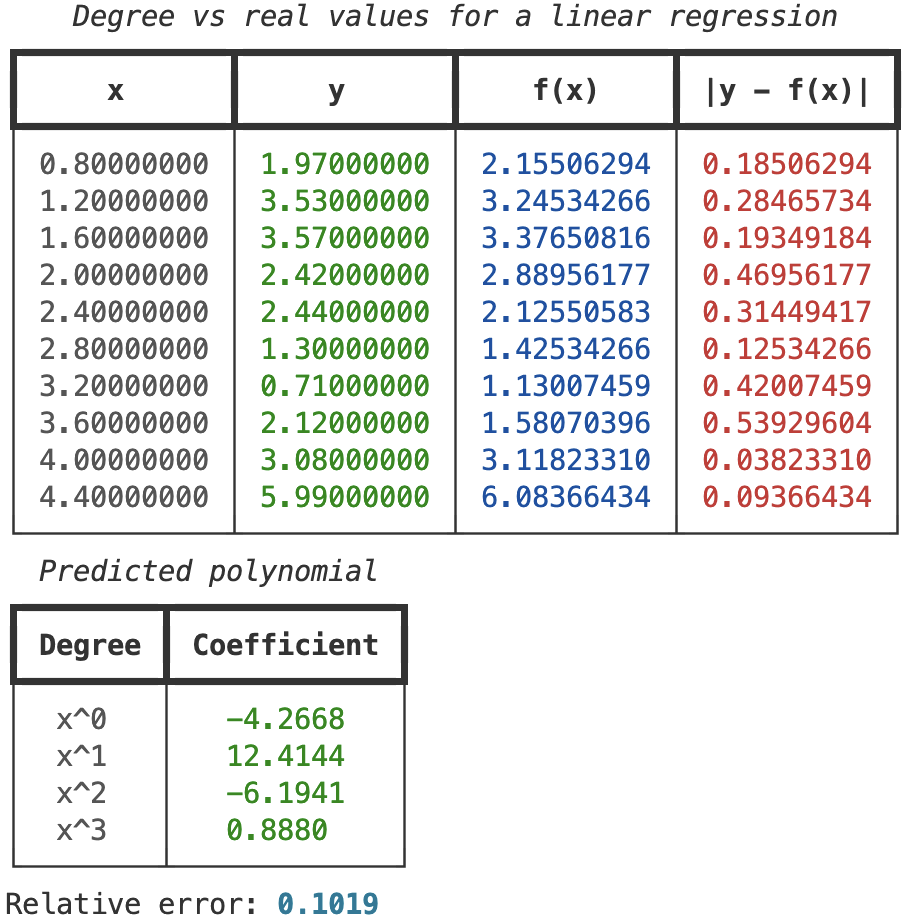
\includegraphics[width=0.5\textwidth]{images/lab_3/table.png}
    \caption{Таблиця з результатами}
    \label{fig:1}
\end{figure}

Бачимо, що поліном має вигляд:
\[
\mathbf{w} \approx \begin{bmatrix}
    -4.267 \\
    12.414 \\
    -6.194 \\
    0.888
\end{bmatrix} \implies f(x;\mathbf{w}) = \mathbf{w}^{\top}\boldsymbol{\phi}(x) \approx 0.888x^3 - 6.194x^2 + 12.414x - 4.267
\]
Відносна похибка вийшла $\Delta \approx 10.2\%$. 

\pagebreak
\subsection{Графік}
Графік, на якому ми зобразили наш побудований поліном:
\begin{figure}[H]
    \centering
    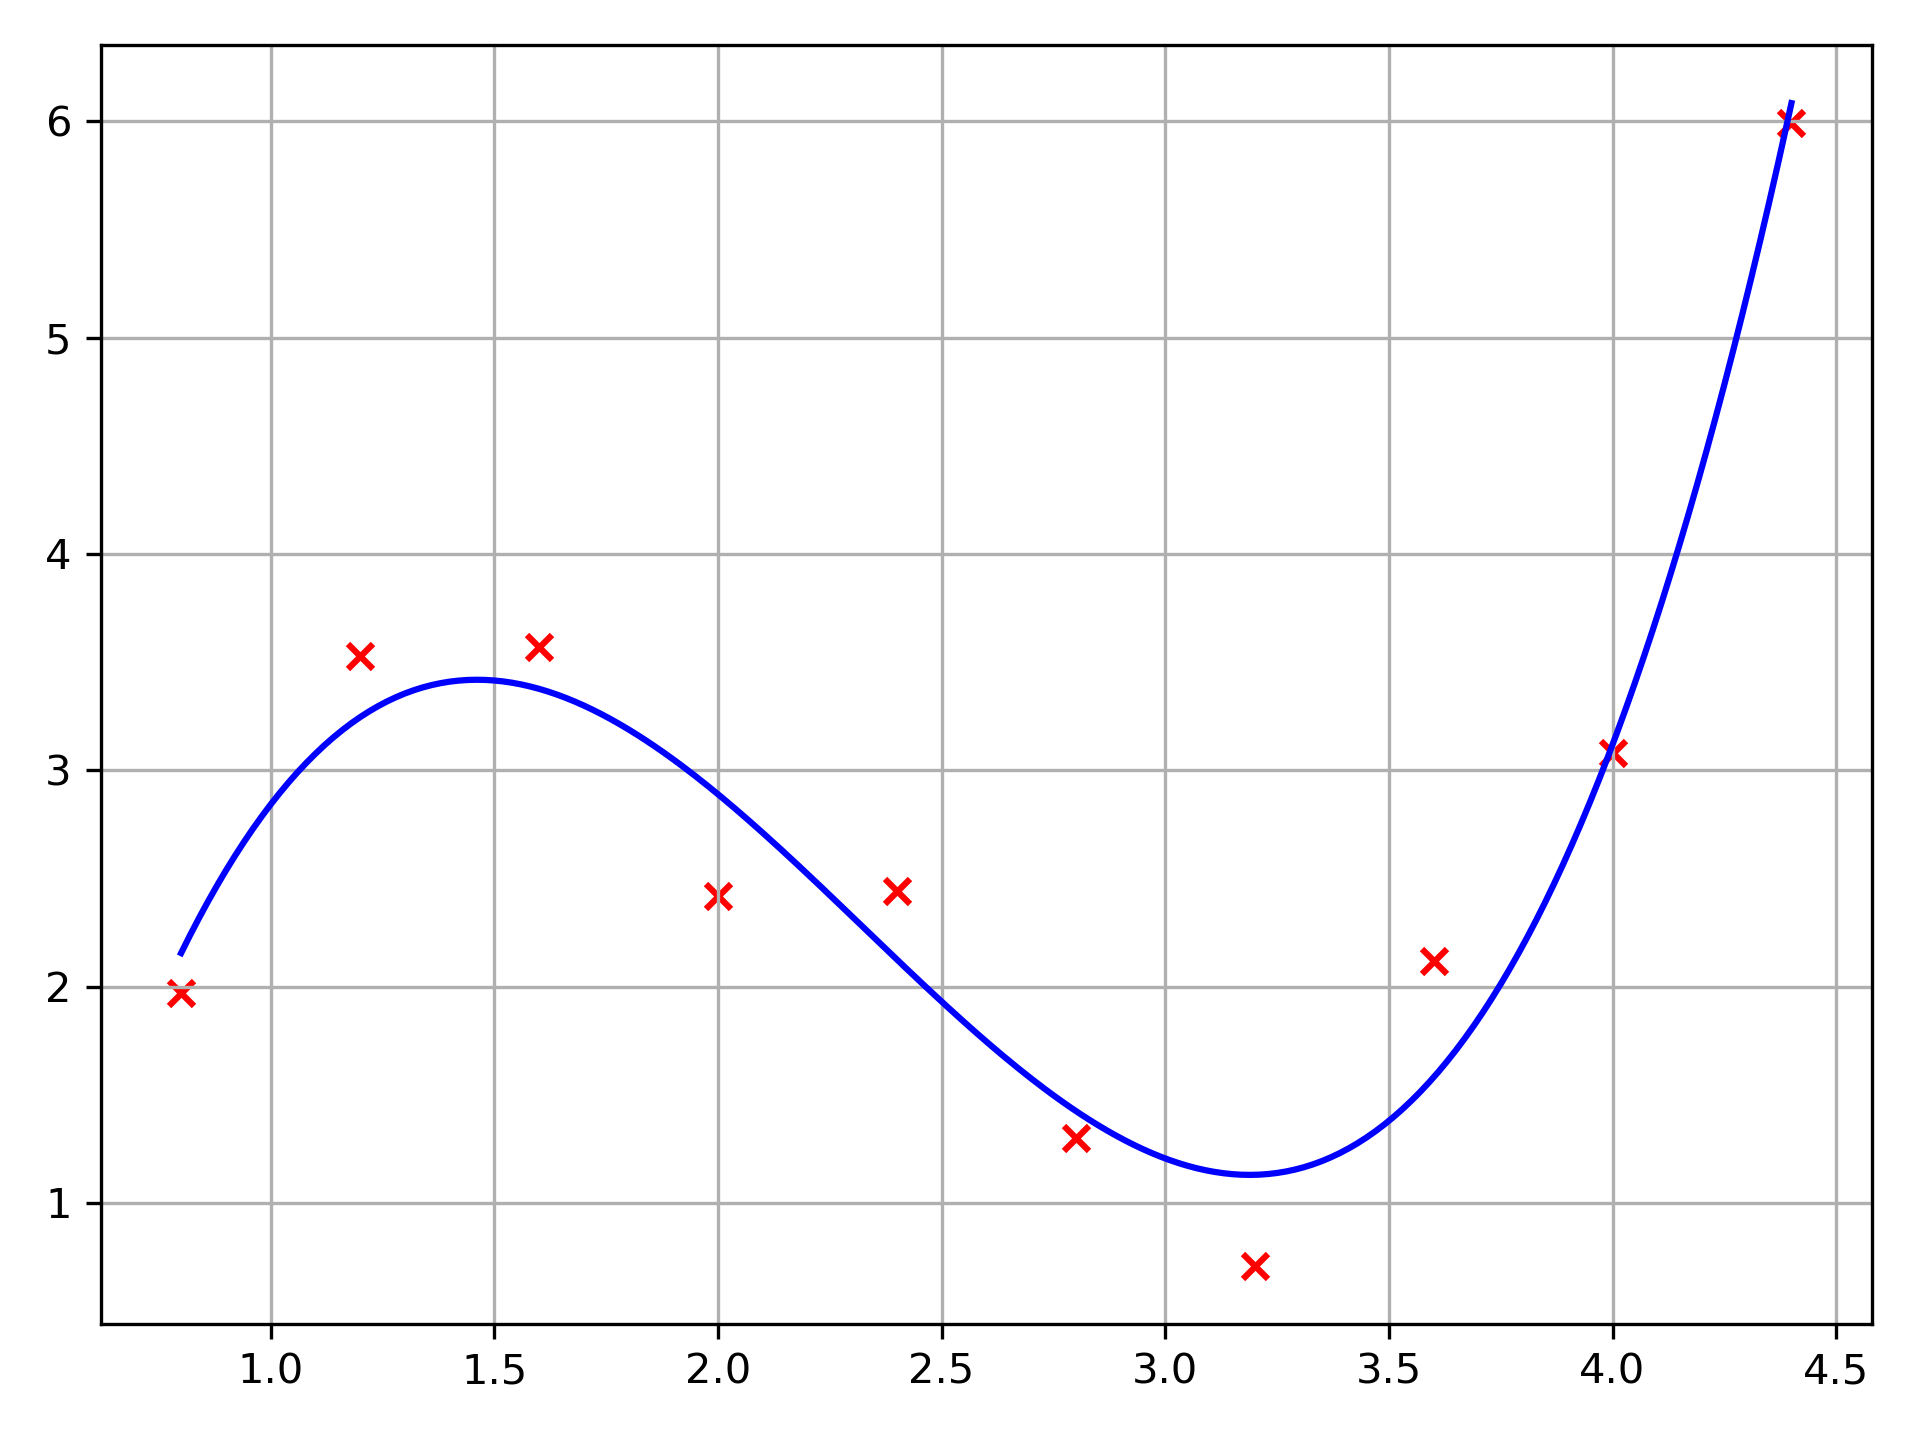
\includegraphics[width=0.6\textwidth]{images/lab_3/plot.png}
    \caption{\textcolor{blue}{Синім} ми зобразили графік $f(x;\mathbf{w})$, а \textcolor{red}{червоним} набір данних}
    \label{fig:3}
\end{figure}
Для перевірки, додатково побудуємо поліноми різних ступенів:
\begin{figure}[H]
    \centering
    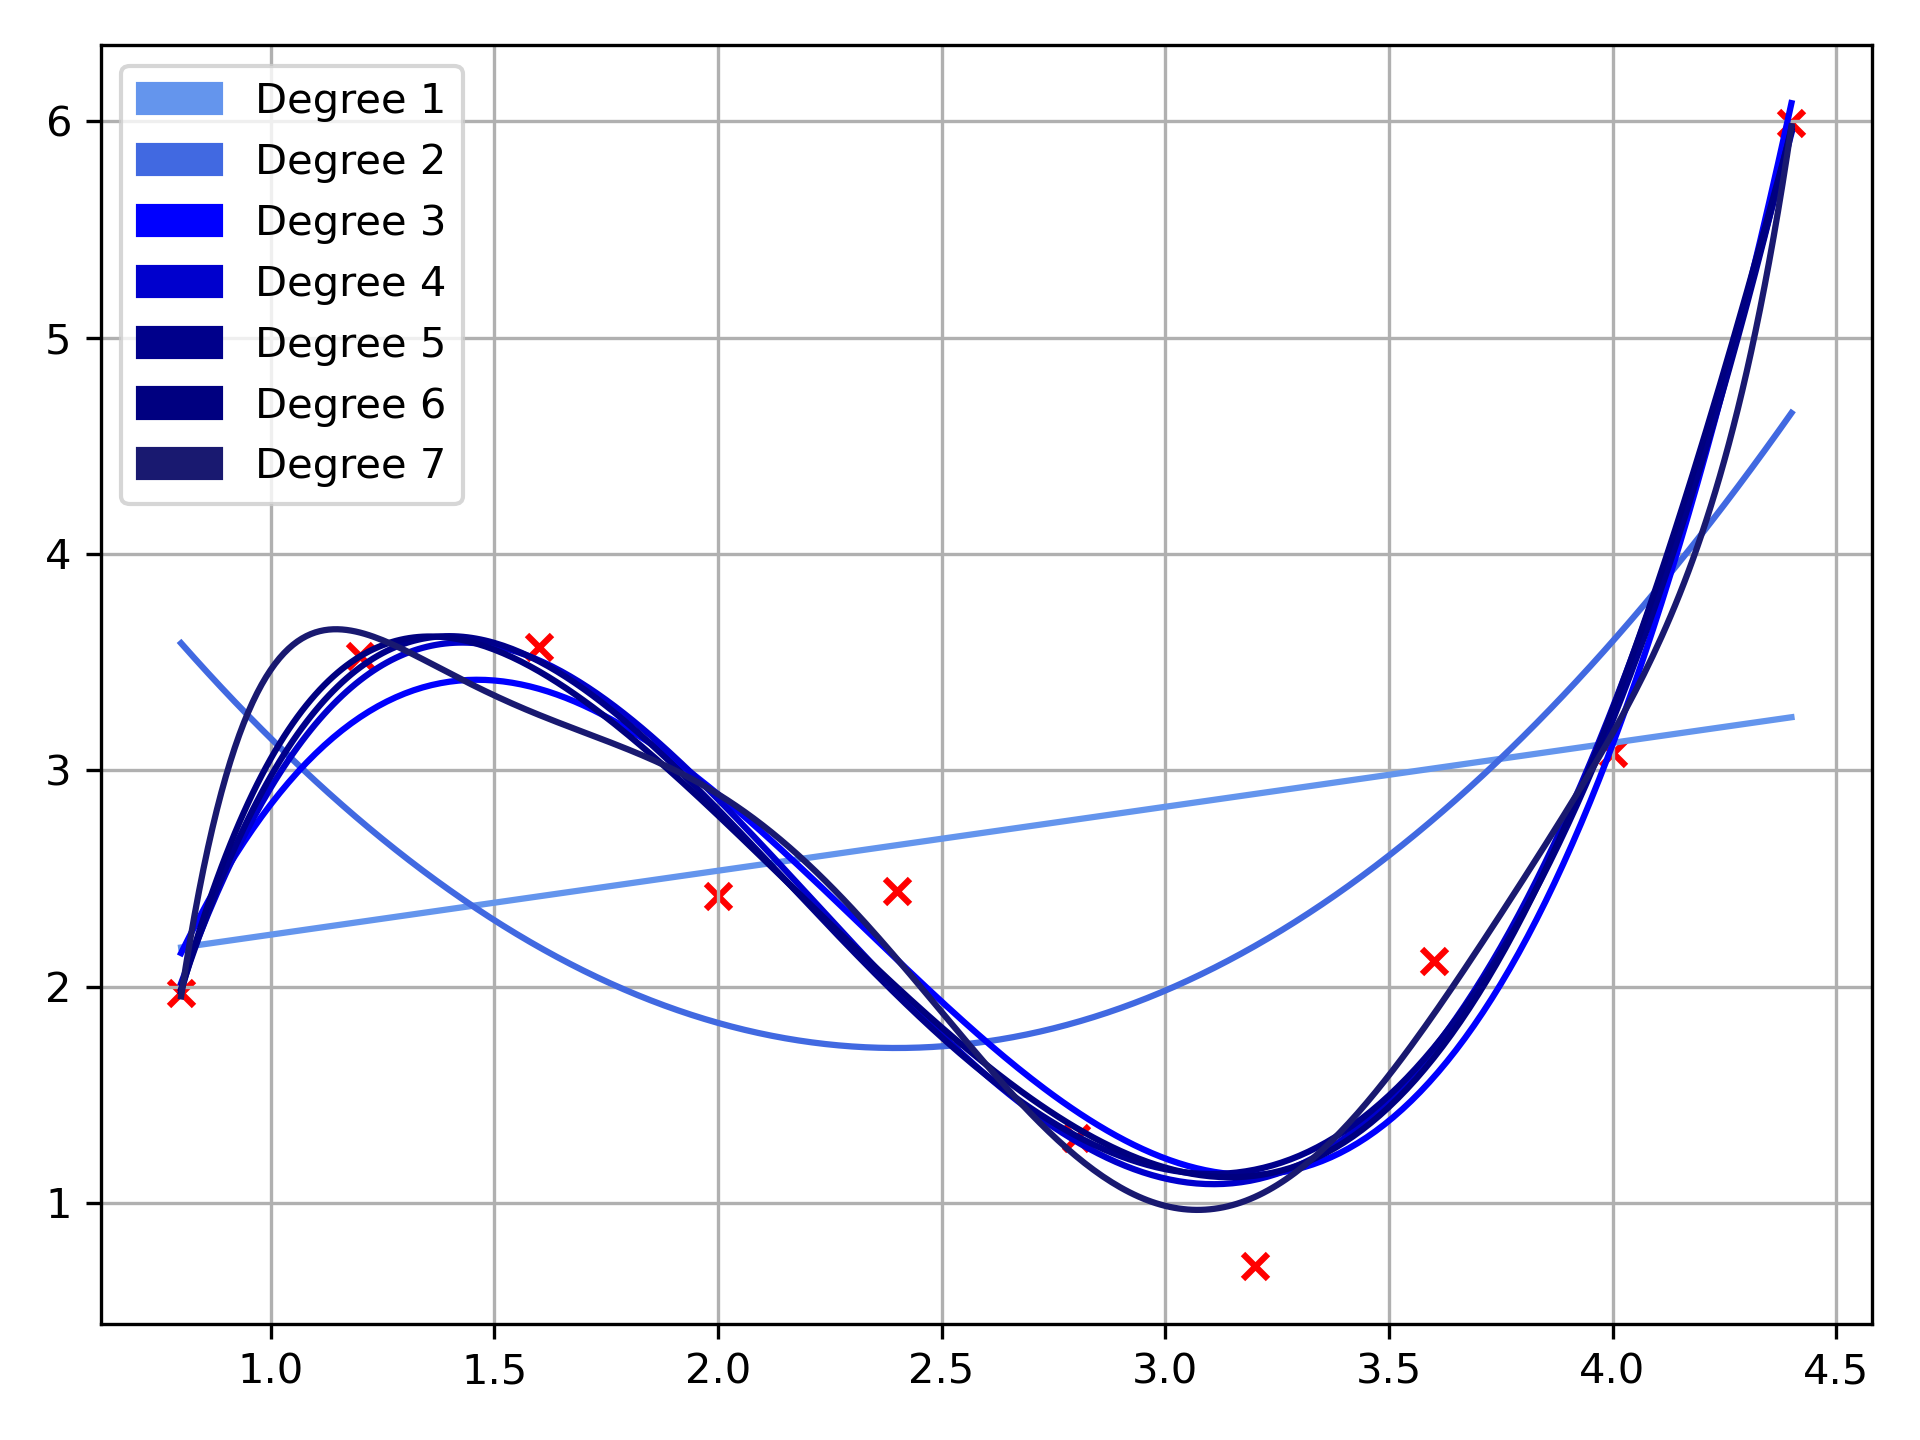
\includegraphics[width=0.6\textwidth]{images/lab_3/degrees.png}
    \caption{Різними відтінками \textcolor{blue}{синього} ми помітили різні ступені $f(x;\mathbf{w})$}
    \label{fig:3}
\end{figure}

\pagebreak
\section{Висновки}

В цій лабораторній роботі ми:
\begin{itemize}
\item навчилися будувати поліном, котрий апроксимує набір точок за допомогою методу найближчих квадратів.
\item навчилися писати комп'ютерну програму (на прикладі мови \texttt{Python}), що будує поліном за методом найближчих квадратів з можливістю обрання ступені поліному та задаванням довільного розміру початкових данних.
\item Оцінювати написану програму (ми це зробили у випадку $\text{deg} \, f(x;\mathbf{w}) = 3$).
\item Візуалізовувати графік та набір точок.
\end{itemize}

Щодо \textit{LSE} методу можемо зробити наступні зауваження:
\begin{enumerate}
    \item В порівнянні з минулими методами інтерполяції (поліном Лагранжа, сплайни тощо), точність на заданому наборі виявилась меньшою. Проте, це ніяк не каже про те, що метод найменьших квадратів є гіршим. Навпаки -- на великому наборі данних, точна інтерполяція часто дає дуже нестабільні результати на проміжках між вузлами, оскільки для інтерполяції нам потрібно поліном ступеня $n_{\mathcal{D}}-1$, навіть якщо ми дуже впевнені про, скажімо, лінійну залежність $y(x)$.
    \item Для \textit{LSE} методу ми розв'язуємо лінійну систему $\mathbf{X}^{\top}\mathbf{X}\hat{\mathbf{w}} = \mathbf{X}^{\top} \mathbf{y}$ за допомогою знаходження оберненої матриці $(\mathbf{X}^{\top}\mathbf{X})^{-1}$, проте з цією операцією є безліч проблем. Існує багато інших більш точних чисельних методів лінійної алгебри для цього. Як альтернатива, найбільш очевидний спосіб -- це метод градієнтного спуску. У найпростішому випадку, ми на кожному кроці знаходимо:
    \[
    \mathbf{w}^{\langle i+1\rangle} \gets \mathbf{w}^{\langle i\rangle} - \eta \frac{\partial \mathcal{L}(\mathbf{w}^{\langle i \rangle} \mid \mathcal{D})}{\partial \mathbf{w}}, \; \eta \ll 1
    \]
    \item Для цього конкретно набору данних, значно меньшу похибку дала би степінь полінома $8$. Проте, з цього набору точок видно, що скоріше за все залежність кубічна. Хоча поліном $8$ ступеня і ближче підігнав криву до них, це б не означало, що якщо ми додамо до набору інші точки, то наша функція би їх добре наближала. У машинному навчанні таке явище називають \textit{overfitting}'ом. 
\end{enumerate}

\end{document}
